\documentclass{beamer}
\usepackage{tikz}
\usetikzlibrary{trees,arrows}

\usetheme{CMU}

\title{AutoMerge}
\subtitle{}
\date{\today}
\author{Francisco Fonseca \and Octavio Mesner}
\institute{Carnegie Mellon University}

\begin{document}
\maketitle

\section{}
\begin{frame}
\frametitle{Goals}
Discuss
\begin{itemize}
\item Project Overview
\item Data
\item Describe Lasso
\item Possible causal pathways
\end{itemize}
\end{frame}

\section{MOMS Data}

\begin{frame}
  \frametitle{MOMS Data}
  \framesubtitle{Overview}
  \begin{itemize}
  \item 744 subject observations
  \item 352 covariates collected
  \item 121 variables with $>$70\% missing (from substudy?)
  \item 57 (8\%) preterm births/629(92\%) full term (58 missing)
  \end{itemize}
\end{frame}

\begin{frame}
  \frametitle{Missing Data}
  \centering
  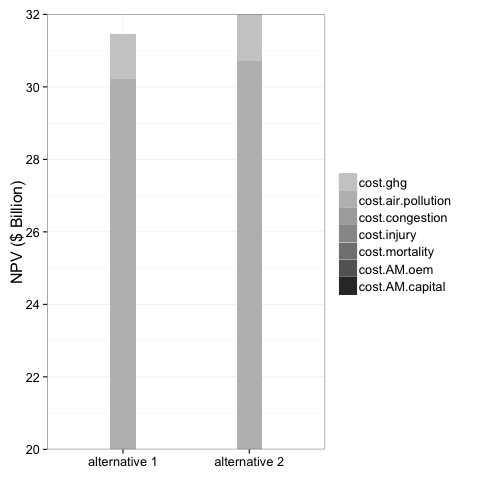
\includegraphics[width=0.75\textwidth]{../../R/barplot1}
\end{frame}

\section{Methods}

\subsection{Evaluation}
\begin{frame}
  \frametitle{Cross Validation}
  How well does a model perform on new data?
  \centering
  %\includegraphics[width=0.9\textwidth]{10foldCv}
\end{frame}

\subsection{Lasso}
\begin{frame}
  \frametitle{What is Lasso?}
  \begin{itemize}
    \item Builds on multiple linear regression
    \item Includes a penalty term for size of parameters
  \end{itemize}
  \centering
  %\includegraphics[width=0.6\textwidth]{lassoPlot}
\end{frame}

\end{document}
